\documentclass[tikz,12pt,border=2pt]{standalone}
\usepackage[T1]{fontenc}
\usepackage[scaled=0.92]{helvet}
\renewcommand{\familydefault}{\sfdefault}
\usetikzlibrary{calc}
\definecolor{cexf}{RGB}{31,84,140}
\definecolor{cimp}{RGB}{179,38,30}
\definecolor{cdex}{RGB}{168,116,26}
\definecolor{cnon}{RGB}{111,78,156}
\definecolor{cagg}{RGB}{58,125,68}
\definecolor{cbase}{RGB}{122,122,122}
\begin{document}
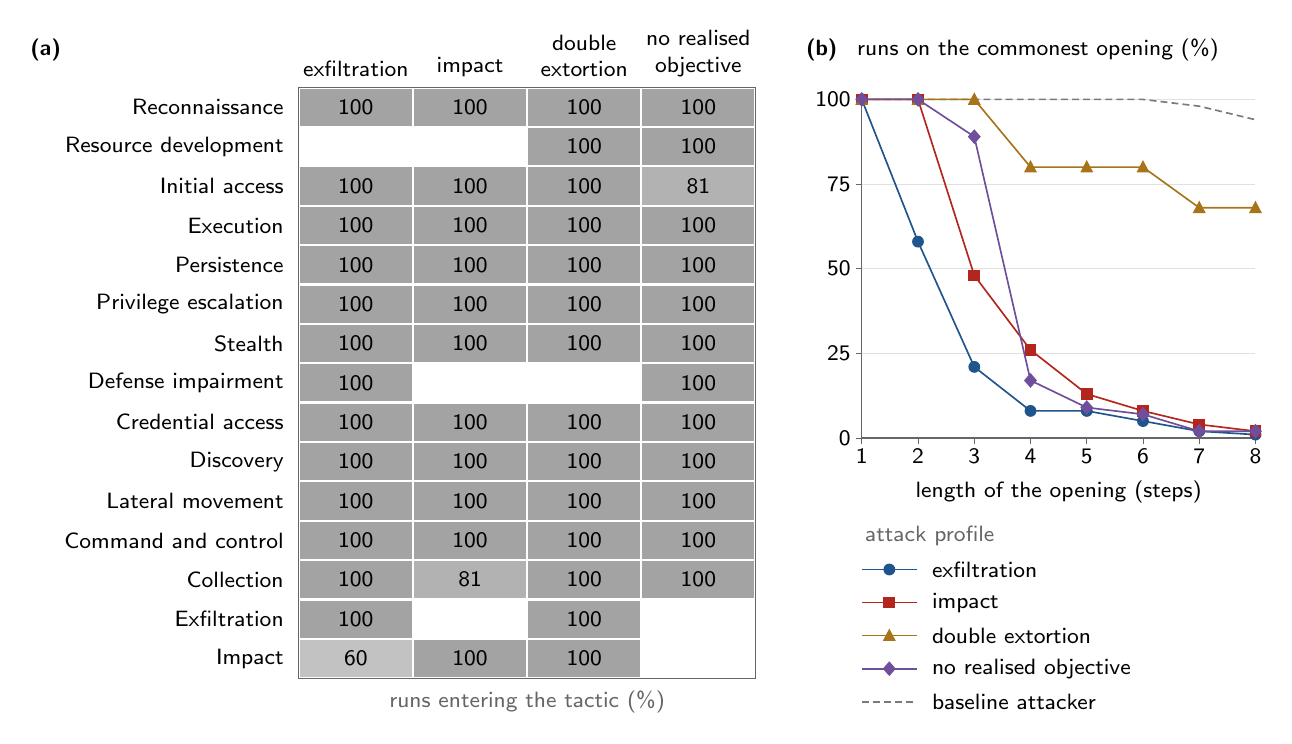
\begin{tikzpicture}[x=1cm,y=1cm,every node/.style={inner sep=1pt,font=\footnotesize}]
\node[anchor=south west,font=\footnotesize\bfseries] at (0,7.800) {(a)};
\node[anchor=south,align=center] at (4.175,7.600) {exfiltration};
\node[anchor=south,align=center] at (5.625,7.600) {impact};
\node[anchor=south,align=center] at (7.075,7.600) {double\\extortion};
\node[anchor=south,align=center] at (8.525,7.600) {no realised\\objective};
\node[anchor=east] at (3.300,7.250) {Reconnaissance};
\fill[black!36] (3.450,7.000) rectangle ++(1.450,0.500);
\node at (4.175,7.250) {100};
\draw[white,line width=0.8pt] (3.450,7.000) rectangle ++(1.450,0.500);
\fill[black!36] (4.900,7.000) rectangle ++(1.450,0.500);
\node at (5.625,7.250) {100};
\draw[white,line width=0.8pt] (4.900,7.000) rectangle ++(1.450,0.500);
\fill[black!36] (6.350,7.000) rectangle ++(1.450,0.500);
\node at (7.075,7.250) {100};
\draw[white,line width=0.8pt] (6.350,7.000) rectangle ++(1.450,0.500);
\fill[black!36] (7.800,7.000) rectangle ++(1.450,0.500);
\node at (8.525,7.250) {100};
\draw[white,line width=0.8pt] (7.800,7.000) rectangle ++(1.450,0.500);
\node[anchor=east] at (3.300,6.750) {Resource development};
\fill[white] (3.450,6.500) rectangle ++(1.450,0.500);
\draw[white,line width=0.8pt] (3.450,6.500) rectangle ++(1.450,0.500);
\fill[white] (4.900,6.500) rectangle ++(1.450,0.500);
\draw[white,line width=0.8pt] (4.900,6.500) rectangle ++(1.450,0.500);
\fill[black!36] (6.350,6.500) rectangle ++(1.450,0.500);
\node at (7.075,6.750) {100};
\draw[white,line width=0.8pt] (6.350,6.500) rectangle ++(1.450,0.500);
\fill[black!36] (7.800,6.500) rectangle ++(1.450,0.500);
\node at (8.525,6.750) {100};
\draw[white,line width=0.8pt] (7.800,6.500) rectangle ++(1.450,0.500);
\node[anchor=east] at (3.300,6.250) {Initial access};
\fill[black!36] (3.450,6.000) rectangle ++(1.450,0.500);
\node at (4.175,6.250) {100};
\draw[white,line width=0.8pt] (3.450,6.000) rectangle ++(1.450,0.500);
\fill[black!36] (4.900,6.000) rectangle ++(1.450,0.500);
\node at (5.625,6.250) {100};
\draw[white,line width=0.8pt] (4.900,6.000) rectangle ++(1.450,0.500);
\fill[black!36] (6.350,6.000) rectangle ++(1.450,0.500);
\node at (7.075,6.250) {100};
\draw[white,line width=0.8pt] (6.350,6.000) rectangle ++(1.450,0.500);
\fill[black!30] (7.800,6.000) rectangle ++(1.450,0.500);
\node at (8.525,6.250) {81};
\draw[white,line width=0.8pt] (7.800,6.000) rectangle ++(1.450,0.500);
\node[anchor=east] at (3.300,5.750) {Execution};
\fill[black!36] (3.450,5.500) rectangle ++(1.450,0.500);
\node at (4.175,5.750) {100};
\draw[white,line width=0.8pt] (3.450,5.500) rectangle ++(1.450,0.500);
\fill[black!36] (4.900,5.500) rectangle ++(1.450,0.500);
\node at (5.625,5.750) {100};
\draw[white,line width=0.8pt] (4.900,5.500) rectangle ++(1.450,0.500);
\fill[black!36] (6.350,5.500) rectangle ++(1.450,0.500);
\node at (7.075,5.750) {100};
\draw[white,line width=0.8pt] (6.350,5.500) rectangle ++(1.450,0.500);
\fill[black!36] (7.800,5.500) rectangle ++(1.450,0.500);
\node at (8.525,5.750) {100};
\draw[white,line width=0.8pt] (7.800,5.500) rectangle ++(1.450,0.500);
\node[anchor=east] at (3.300,5.250) {Persistence};
\fill[black!36] (3.450,5.000) rectangle ++(1.450,0.500);
\node at (4.175,5.250) {100};
\draw[white,line width=0.8pt] (3.450,5.000) rectangle ++(1.450,0.500);
\fill[black!36] (4.900,5.000) rectangle ++(1.450,0.500);
\node at (5.625,5.250) {100};
\draw[white,line width=0.8pt] (4.900,5.000) rectangle ++(1.450,0.500);
\fill[black!36] (6.350,5.000) rectangle ++(1.450,0.500);
\node at (7.075,5.250) {100};
\draw[white,line width=0.8pt] (6.350,5.000) rectangle ++(1.450,0.500);
\fill[black!36] (7.800,5.000) rectangle ++(1.450,0.500);
\node at (8.525,5.250) {100};
\draw[white,line width=0.8pt] (7.800,5.000) rectangle ++(1.450,0.500);
\node[anchor=east] at (3.300,4.750) {Privilege escalation};
\fill[black!36] (3.450,4.500) rectangle ++(1.450,0.500);
\node at (4.175,4.750) {100};
\draw[white,line width=0.8pt] (3.450,4.500) rectangle ++(1.450,0.500);
\fill[black!36] (4.900,4.500) rectangle ++(1.450,0.500);
\node at (5.625,4.750) {100};
\draw[white,line width=0.8pt] (4.900,4.500) rectangle ++(1.450,0.500);
\fill[black!36] (6.350,4.500) rectangle ++(1.450,0.500);
\node at (7.075,4.750) {100};
\draw[white,line width=0.8pt] (6.350,4.500) rectangle ++(1.450,0.500);
\fill[black!36] (7.800,4.500) rectangle ++(1.450,0.500);
\node at (8.525,4.750) {100};
\draw[white,line width=0.8pt] (7.800,4.500) rectangle ++(1.450,0.500);
\node[anchor=east] at (3.300,4.250) {Stealth};
\fill[black!36] (3.450,4.000) rectangle ++(1.450,0.500);
\node at (4.175,4.250) {100};
\draw[white,line width=0.8pt] (3.450,4.000) rectangle ++(1.450,0.500);
\fill[black!36] (4.900,4.000) rectangle ++(1.450,0.500);
\node at (5.625,4.250) {100};
\draw[white,line width=0.8pt] (4.900,4.000) rectangle ++(1.450,0.500);
\fill[black!36] (6.350,4.000) rectangle ++(1.450,0.500);
\node at (7.075,4.250) {100};
\draw[white,line width=0.8pt] (6.350,4.000) rectangle ++(1.450,0.500);
\fill[black!36] (7.800,4.000) rectangle ++(1.450,0.500);
\node at (8.525,4.250) {100};
\draw[white,line width=0.8pt] (7.800,4.000) rectangle ++(1.450,0.500);
\node[anchor=east] at (3.300,3.750) {Defense impairment};
\fill[black!36] (3.450,3.500) rectangle ++(1.450,0.500);
\node at (4.175,3.750) {100};
\draw[white,line width=0.8pt] (3.450,3.500) rectangle ++(1.450,0.500);
\fill[white] (4.900,3.500) rectangle ++(1.450,0.500);
\draw[white,line width=0.8pt] (4.900,3.500) rectangle ++(1.450,0.500);
\fill[white] (6.350,3.500) rectangle ++(1.450,0.500);
\draw[white,line width=0.8pt] (6.350,3.500) rectangle ++(1.450,0.500);
\fill[black!36] (7.800,3.500) rectangle ++(1.450,0.500);
\node at (8.525,3.750) {100};
\draw[white,line width=0.8pt] (7.800,3.500) rectangle ++(1.450,0.500);
\node[anchor=east] at (3.300,3.250) {Credential access};
\fill[black!36] (3.450,3.000) rectangle ++(1.450,0.500);
\node at (4.175,3.250) {100};
\draw[white,line width=0.8pt] (3.450,3.000) rectangle ++(1.450,0.500);
\fill[black!36] (4.900,3.000) rectangle ++(1.450,0.500);
\node at (5.625,3.250) {100};
\draw[white,line width=0.8pt] (4.900,3.000) rectangle ++(1.450,0.500);
\fill[black!36] (6.350,3.000) rectangle ++(1.450,0.500);
\node at (7.075,3.250) {100};
\draw[white,line width=0.8pt] (6.350,3.000) rectangle ++(1.450,0.500);
\fill[black!36] (7.800,3.000) rectangle ++(1.450,0.500);
\node at (8.525,3.250) {100};
\draw[white,line width=0.8pt] (7.800,3.000) rectangle ++(1.450,0.500);
\node[anchor=east] at (3.300,2.750) {Discovery};
\fill[black!36] (3.450,2.500) rectangle ++(1.450,0.500);
\node at (4.175,2.750) {100};
\draw[white,line width=0.8pt] (3.450,2.500) rectangle ++(1.450,0.500);
\fill[black!36] (4.900,2.500) rectangle ++(1.450,0.500);
\node at (5.625,2.750) {100};
\draw[white,line width=0.8pt] (4.900,2.500) rectangle ++(1.450,0.500);
\fill[black!36] (6.350,2.500) rectangle ++(1.450,0.500);
\node at (7.075,2.750) {100};
\draw[white,line width=0.8pt] (6.350,2.500) rectangle ++(1.450,0.500);
\fill[black!36] (7.800,2.500) rectangle ++(1.450,0.500);
\node at (8.525,2.750) {100};
\draw[white,line width=0.8pt] (7.800,2.500) rectangle ++(1.450,0.500);
\node[anchor=east] at (3.300,2.250) {Lateral movement};
\fill[black!36] (3.450,2.000) rectangle ++(1.450,0.500);
\node at (4.175,2.250) {100};
\draw[white,line width=0.8pt] (3.450,2.000) rectangle ++(1.450,0.500);
\fill[black!36] (4.900,2.000) rectangle ++(1.450,0.500);
\node at (5.625,2.250) {100};
\draw[white,line width=0.8pt] (4.900,2.000) rectangle ++(1.450,0.500);
\fill[black!36] (6.350,2.000) rectangle ++(1.450,0.500);
\node at (7.075,2.250) {100};
\draw[white,line width=0.8pt] (6.350,2.000) rectangle ++(1.450,0.500);
\fill[black!36] (7.800,2.000) rectangle ++(1.450,0.500);
\node at (8.525,2.250) {100};
\draw[white,line width=0.8pt] (7.800,2.000) rectangle ++(1.450,0.500);
\node[anchor=east] at (3.300,1.750) {Command and control};
\fill[black!36] (3.450,1.500) rectangle ++(1.450,0.500);
\node at (4.175,1.750) {100};
\draw[white,line width=0.8pt] (3.450,1.500) rectangle ++(1.450,0.500);
\fill[black!36] (4.900,1.500) rectangle ++(1.450,0.500);
\node at (5.625,1.750) {100};
\draw[white,line width=0.8pt] (4.900,1.500) rectangle ++(1.450,0.500);
\fill[black!36] (6.350,1.500) rectangle ++(1.450,0.500);
\node at (7.075,1.750) {100};
\draw[white,line width=0.8pt] (6.350,1.500) rectangle ++(1.450,0.500);
\fill[black!36] (7.800,1.500) rectangle ++(1.450,0.500);
\node at (8.525,1.750) {100};
\draw[white,line width=0.8pt] (7.800,1.500) rectangle ++(1.450,0.500);
\node[anchor=east] at (3.300,1.250) {Collection};
\fill[black!36] (3.450,1.000) rectangle ++(1.450,0.500);
\node at (4.175,1.250) {100};
\draw[white,line width=0.8pt] (3.450,1.000) rectangle ++(1.450,0.500);
\fill[black!30] (4.900,1.000) rectangle ++(1.450,0.500);
\node at (5.625,1.250) {81};
\draw[white,line width=0.8pt] (4.900,1.000) rectangle ++(1.450,0.500);
\fill[black!36] (6.350,1.000) rectangle ++(1.450,0.500);
\node at (7.075,1.250) {100};
\draw[white,line width=0.8pt] (6.350,1.000) rectangle ++(1.450,0.500);
\fill[black!36] (7.800,1.000) rectangle ++(1.450,0.500);
\node at (8.525,1.250) {100};
\draw[white,line width=0.8pt] (7.800,1.000) rectangle ++(1.450,0.500);
\node[anchor=east] at (3.300,0.750) {Exfiltration};
\fill[black!36] (3.450,0.500) rectangle ++(1.450,0.500);
\node at (4.175,0.750) {100};
\draw[white,line width=0.8pt] (3.450,0.500) rectangle ++(1.450,0.500);
\fill[white] (4.900,0.500) rectangle ++(1.450,0.500);
\draw[white,line width=0.8pt] (4.900,0.500) rectangle ++(1.450,0.500);
\fill[black!36] (6.350,0.500) rectangle ++(1.450,0.500);
\node at (7.075,0.750) {100};
\draw[white,line width=0.8pt] (6.350,0.500) rectangle ++(1.450,0.500);
\fill[white] (7.800,0.500) rectangle ++(1.450,0.500);
\draw[white,line width=0.8pt] (7.800,0.500) rectangle ++(1.450,0.500);
\node[anchor=east] at (3.300,0.250) {Impact};
\fill[black!24] (3.450,0.000) rectangle ++(1.450,0.500);
\node at (4.175,0.250) {60};
\draw[white,line width=0.8pt] (3.450,0.000) rectangle ++(1.450,0.500);
\fill[black!36] (4.900,0.000) rectangle ++(1.450,0.500);
\node at (5.625,0.250) {100};
\draw[white,line width=0.8pt] (4.900,0.000) rectangle ++(1.450,0.500);
\fill[black!36] (6.350,0.000) rectangle ++(1.450,0.500);
\node at (7.075,0.250) {100};
\draw[white,line width=0.8pt] (6.350,0.000) rectangle ++(1.450,0.500);
\fill[white] (7.800,0.000) rectangle ++(1.450,0.500);
\draw[white,line width=0.8pt] (7.800,0.000) rectangle ++(1.450,0.500);
\draw[black!60,line width=0.4pt] (3.450,0.000) rectangle (9.250,7.500);
\node[anchor=north,text=black!60] at (6.350,-0.120) {runs entering the tactic (\%)};
\draw[black!60,line width=0.4pt] (10.600,3.050) -- (15.600,3.050);
\draw[black!60,line width=0.4pt] (10.600,3.050) -- (10.600,7.350);
\draw[black!60,line width=0.3pt] (10.530,3.050) -- (10.600,3.050);
\node[anchor=east] at (10.500,3.050) {0};
\draw[black!60,line width=0.3pt] (10.530,4.125) -- (10.600,4.125);
\draw[black!12,line width=0.2pt] (10.600,4.125) -- (15.600,4.125);
\node[anchor=east] at (10.500,4.125) {25};
\draw[black!60,line width=0.3pt] (10.530,5.200) -- (10.600,5.200);
\draw[black!12,line width=0.2pt] (10.600,5.200) -- (15.600,5.200);
\node[anchor=east] at (10.500,5.200) {50};
\draw[black!60,line width=0.3pt] (10.530,6.275) -- (10.600,6.275);
\draw[black!12,line width=0.2pt] (10.600,6.275) -- (15.600,6.275);
\node[anchor=east] at (10.500,6.275) {75};
\draw[black!60,line width=0.3pt] (10.530,7.350) -- (10.600,7.350);
\draw[black!12,line width=0.2pt] (10.600,7.350) -- (15.600,7.350);
\node[anchor=east] at (10.500,7.350) {100};
\draw[black!60,line width=0.3pt] (10.600,3.050) -- (10.600,2.980);
\node[anchor=north] at (10.600,2.950) {1};
\draw[black!60,line width=0.3pt] (11.314,3.050) -- (11.314,2.980);
\node[anchor=north] at (11.314,2.950) {2};
\draw[black!60,line width=0.3pt] (12.029,3.050) -- (12.029,2.980);
\node[anchor=north] at (12.029,2.950) {3};
\draw[black!60,line width=0.3pt] (12.743,3.050) -- (12.743,2.980);
\node[anchor=north] at (12.743,2.950) {4};
\draw[black!60,line width=0.3pt] (13.457,3.050) -- (13.457,2.980);
\node[anchor=north] at (13.457,2.950) {5};
\draw[black!60,line width=0.3pt] (14.171,3.050) -- (14.171,2.980);
\node[anchor=north] at (14.171,2.950) {6};
\draw[black!60,line width=0.3pt] (14.886,3.050) -- (14.886,2.980);
\node[anchor=north] at (14.886,2.950) {7};
\draw[black!60,line width=0.3pt] (15.600,3.050) -- (15.600,2.980);
\node[anchor=north] at (15.600,2.950) {8};
\node[anchor=north] at (13.100,2.550) {length of the opening (steps)};
\node[anchor=south west,font=\footnotesize\bfseries] at (9.850,7.800) {(b)};
\node[anchor=south west] at (10.500,7.800) {runs on the commonest opening (\%)};
\draw[cbase,line width=0.6pt,dash pattern=on 2.5pt off 1.5pt] (10.600,7.350) -- (11.314,7.350) -- (12.029,7.350) -- (12.743,7.350) -- (13.457,7.350) -- (14.171,7.350) -- (14.886,7.264) -- (15.600,7.092);
\draw[cexf,line width=0.6pt] (10.600,7.350) -- (11.314,5.544) -- (12.029,3.953) -- (12.743,3.394) -- (13.457,3.394) -- (14.171,3.265) -- (14.886,3.136) -- (15.600,3.093);
\fill[cexf] (10.600,7.350) circle (0.075cm);
\fill[cexf] (11.314,5.544) circle (0.075cm);
\fill[cexf] (12.029,3.953) circle (0.075cm);
\fill[cexf] (12.743,3.394) circle (0.075cm);
\fill[cexf] (13.457,3.394) circle (0.075cm);
\fill[cexf] (14.171,3.265) circle (0.075cm);
\fill[cexf] (14.886,3.136) circle (0.075cm);
\fill[cexf] (15.600,3.093) circle (0.075cm);
\draw[cimp,line width=0.6pt] (10.600,7.350) -- (11.314,7.350) -- (12.029,5.114) -- (12.743,4.168) -- (13.457,3.609) -- (14.171,3.394) -- (14.886,3.222) -- (15.600,3.136);
\fill[cimp] (10.600,7.350) ++(-0.075,-0.075) rectangle ++(0.150,0.150);
\fill[cimp] (11.314,7.350) ++(-0.075,-0.075) rectangle ++(0.150,0.150);
\fill[cimp] (12.029,5.114) ++(-0.075,-0.075) rectangle ++(0.150,0.150);
\fill[cimp] (12.743,4.168) ++(-0.075,-0.075) rectangle ++(0.150,0.150);
\fill[cimp] (13.457,3.609) ++(-0.075,-0.075) rectangle ++(0.150,0.150);
\fill[cimp] (14.171,3.394) ++(-0.075,-0.075) rectangle ++(0.150,0.150);
\fill[cimp] (14.886,3.222) ++(-0.075,-0.075) rectangle ++(0.150,0.150);
\fill[cimp] (15.600,3.136) ++(-0.075,-0.075) rectangle ++(0.150,0.150);
\draw[cdex,line width=0.6pt] (10.600,7.350) -- (11.314,7.350) -- (12.029,7.350) -- (12.743,6.490) -- (13.457,6.490) -- (14.171,6.490) -- (14.886,5.974) -- (15.600,5.974);
\fill[cdex] (10.518,7.282) -- (10.682,7.282) -- (10.600,7.440) -- cycle;
\fill[cdex] (11.232,7.282) -- (11.397,7.282) -- (11.314,7.440) -- cycle;
\fill[cdex] (11.946,7.282) -- (12.111,7.282) -- (12.029,7.440) -- cycle;
\fill[cdex] (12.660,6.423) -- (12.825,6.423) -- (12.743,6.580) -- cycle;
\fill[cdex] (13.375,6.423) -- (13.540,6.423) -- (13.457,6.580) -- cycle;
\fill[cdex] (14.089,6.423) -- (14.254,6.423) -- (14.171,6.580) -- cycle;
\fill[cdex] (14.803,5.907) -- (14.968,5.907) -- (14.886,6.064) -- cycle;
\fill[cdex] (15.518,5.907) -- (15.682,5.907) -- (15.600,6.064) -- cycle;
\draw[cnon,line width=0.6pt] (10.600,7.350) -- (11.314,7.350) -- (12.029,6.877) -- (12.743,3.781) -- (13.457,3.437) -- (14.171,3.351) -- (14.886,3.136) -- (15.600,3.136);
\fill[cnon] (10.600,7.444) -- (10.682,7.350) -- (10.600,7.256) -- (10.518,7.350) -- cycle;
\fill[cnon] (11.314,7.444) -- (11.397,7.350) -- (11.314,7.256) -- (11.232,7.350) -- cycle;
\fill[cnon] (12.029,6.971) -- (12.111,6.877) -- (12.029,6.783) -- (11.946,6.877) -- cycle;
\fill[cnon] (12.743,3.875) -- (12.825,3.781) -- (12.743,3.687) -- (12.660,3.781) -- cycle;
\fill[cnon] (13.457,3.531) -- (13.540,3.437) -- (13.457,3.343) -- (13.375,3.437) -- cycle;
\fill[cnon] (14.171,3.445) -- (14.254,3.351) -- (14.171,3.257) -- (14.089,3.351) -- cycle;
\fill[cnon] (14.886,3.230) -- (14.968,3.136) -- (14.886,3.042) -- (14.803,3.136) -- cycle;
\fill[cnon] (15.600,3.230) -- (15.682,3.136) -- (15.600,3.042) -- (15.518,3.136) -- cycle;
\node[anchor=west,text=black!60] at (10.600,1.800) {attack profile};
\draw[cexf,line width=0.6pt] (10.600,1.380) -- (11.300,1.380);
\fill[cexf] (10.950,1.380) circle (0.075cm);
\node[anchor=west] at (11.450,1.380) {exfiltration};
\draw[cimp,line width=0.6pt] (10.600,0.960) -- (11.300,0.960);
\fill[cimp] (10.950,0.960) ++(-0.075,-0.075) rectangle ++(0.150,0.150);
\node[anchor=west] at (11.450,0.960) {impact};
\draw[cdex,line width=0.6pt] (10.600,0.540) -- (11.300,0.540);
\fill[cdex] (10.867,0.473) -- (11.032,0.473) -- (10.950,0.630) -- cycle;
\node[anchor=west] at (11.450,0.540) {double extortion};
\draw[cnon,line width=0.6pt] (10.600,0.120) -- (11.300,0.120);
\fill[cnon] (10.950,0.214) -- (11.032,0.120) -- (10.950,0.026) -- (10.867,0.120) -- cycle;
\node[anchor=west] at (11.450,0.120) {no realised objective};
\draw[cbase,line width=0.6pt,dash pattern=on 2.5pt off 1.5pt] (10.600,-0.300) -- (11.300,-0.300);
\node[anchor=west] at (11.450,-0.300) {baseline attacker};
\end{tikzpicture}
\end{document}
